\documentclass[runningheads,a4paper]{llncs}

\usepackage{amssymb}
\setcounter{tocdepth}{3}
\usepackage{graphicx}
\usepackage{hyperref}
\usepackage{fixltx2e}

\usepackage{url}
\urldef{\mailsa}\path|{i.c.t.m.speek, a.c.stolwijk}@student.tudelft.nl|
\newcommand{\keywords}[1]{\par\addvspace\baselineskip%
\noindent\keywordname\enspace\ignorespaces#1}

\begin{document}

\mainmatter% start of an individual contribution

% first the title is needed
\title{Presentation Plan\\
FF-Replan: \& RFF\@: Exploiting classical AI planning for uncertain and probabilistic domains}

% a short form should be given in case it is too long for the running head
\titlerunning{Presentation Plan}

\author{I.C.T.M Speek, A.C. Stolwijk}

%
\authorrunning{Presentation Plan Seminar Algorithms FF-replan \& RFF}
% (feature abused for this document to repeat the title also on left hand pages)

% the affiliations are given next; don't give your e-mail address
% unless you accept that it will be published
\institute{Seminar Algorithms, Embedded Software,
Msc Embedded Systems,\\
Delft University of Technology\\
\mailsa\\
}

%\toctitle{Lecture Notes in Computer Science}
%\tocauthor{Authors' Instructions}

\maketitle

\section{Introduction to a planner (A)}

What is a planner? [Will need some more detailing].\\

Examples of planning problems:

\begin{itemize}
	\item Blocks World
	\item Motion Planning
	\item Inventory Management~\cite{puterman2009markov}
	\item Equipment Maintenance~\cite{puterman2009markov}
	\item Communication Models~\cite{puterman2009markov}
\end{itemize}

\begin{figure}[htb]%
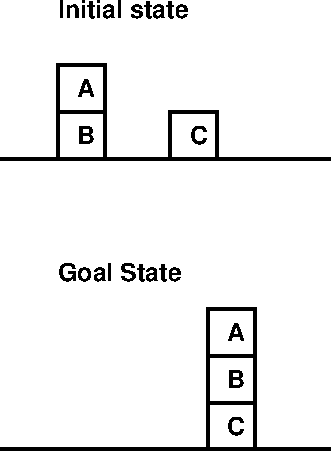
\includegraphics[width=0.4\columnwidth]{blocksworld.pdf}%
\caption{Blocks World example (Figure from~\url{http://www.cs.utexas.edu/~mooney/cs343/slide-handouts/planning.4.pdf})}%
\label{fig:blocksworld}%
\end{figure}

In figure~\ref{fig:blocksworld}, how do you go from the initial state to the
goal state? First you have to move A from B, before you can put B on C and
finally A on B. This is a very trivial example of planning. Between each
action of moving a block, the world is in a certain state. Actions provide
a way to go from one state to another, but from each state, it is possible
to do multiple actions. For example in the initial state you can move C onto
A, but that doesn't help achieving the goal. Finding the right sequence of
actions is what a planner does. From this we can define:

\subsubsection{Inventory Management} How much of X do we need to order from the
supplier every day until the end of the season?

\subsubsection{Equipment Maintenance} A bus company is responsible for keeping
all buses in a good working condition. One aspect is when to replace the bus
engines~\cite{puterman2009markov}. This problem could be represented as a
MDP\@.  When to schedule disruptive maintenance jobs by their deadline?

\subsubsection{Communication Models} Many computer, manufacturing and
communication systems can be modelled as networks with waiting queues and
servers. Systems have receiving packages, routing, and varying service rates.

\noindent \textbf{Planning Problem}:

\begin{itemize}
	\item Initial State
	\item Goal State
	\item Set of actions
	\item Conditions
\end{itemize}

\noindent And the \textbf{Planning Plan}:

\begin{itemize}
	\item Set of actions
	\item Executable in the initial state
	\item Resulting in a state that satisfies the goal state
\end{itemize}

\section{What is uncertainty (I)}

\emph{Uncertainty applies to predictions of future events, to physical measurements that are already made, or to the unknown. Uncertainty arises in partially observable and/or stochastic environments, as well as due to ignorance and/or indolence} [1]. \\

Uncertain (adjective). \\
1. not able to be relied on; not known or definite. [2]

In the rest of this topic discuss the different domains and applications.

\subsection{Real world examples}

Growing plants is an extremely uncertain domain. When everything goes well, it should be fine to water it once a week. However my room environment has proven to be an uncertain domain where wind, temperature and sunlight severely impacts my ability to plan for nurturing my plants.

\subsection{Embedded Systems in uncertain domains}

Cruise control (stabilizing systems), quad rotor, AI, robots

\subsection{Benchmarking for uncertain domains}

Traffic control benchmark for the 2014 IPCC probabilistic continuous domain.
Tidybot: a housecleaning robot [3]. \\

\noindent [1] [Wikipedia http://en.wikipedia.org/wiki/Uncertainty]
[2] [Google definition]
[3] [http://www.plg.inf.uc3m.es/ipc2011-deterministic/DomainsSequential.html\#Barman]

\section{Historical background information}
A swift introduction to the evolution of planning algorithms. For every problem state the:
\begin{itemize}
	\item The problem definition
	\item The motivation for the solution
	\item The strengths
	\item The weaknesses
\end{itemize}

\subsection{Classical Planners}

Classical Planners do not take uncertainties into account. Classical Planners
are deterministic.

STRIPS is considered one of the first planning algorithms and
representations.~\cite{lavalle2006planning}. It is a very simple logic based
only on literal. It's very nice to describe planning problems in a
descriptive way that closely corresponds to the application. Also due to the
operator definition (action/preconditions) it's possible to describe complex


\subsection{Planning graphs}

With states and actions, it's easy to see that a planning problem can be
represented by a directed graph, where the states are the nodes, and the
actions are the edges that connect states. The planning problem is now
a search problem from the root to the goal states.

A well known planner that uses a planning graph is Graphplan.
[However that seems, after some investigation, to work in an interesting
different way\ldots]

\subsection{Planning as a satisfiability}

\subsection{Heuristic search Planning (HSP)}

\subsection{FF Planner (I)}
Use this: \cite{Hoffmann01theff}

\subsection{Markov Decision Processes}

State what's \cite{monahan1982state} is saying about the state of the art MDPs
in the 1980s.

\noindent A Markov Decision Process has the form $M = (S, A, app, Pr, R)$

\begin{itemize}
	\item $S$ and $A$ are the finite set of states and actions
	\item $app(s)$ is the set of of actions applicable in $s$
	\item For every $a \in app(s)$, $Pr(s,a,s')$ is the probability of a state
		transition from $s$ to $s'$
	\item $R(s,a,s')$ is the \emph{reward} of the transition $(s,a,s')$.
\end{itemize}

\subsubsection{Shortcomings MDPs}
\begin{itemize}
	\item Is computationally challenging as it tries to optimize large parts of the policy at once
\end{itemize}

\section{Planning under uncertainty}

\subsection{FF-replan \cite{FFReplan}}
%Define the problem considering probabilistic and deterministic planning

\subsubsection{Problem definition}
Probabilistic planning is naturally formulated using Markov Decision Processes. These probabilistic planners focus on the entire state space. Deterministic planning has developed heuristic functions enabling exploration of restricted portions of the state space enroute to the goal state. This enables the planner to account for unexpected states rather than ending up in a dead-end. MDP's had been the standard in planning algorithms [FOR HOW LONG]? However by relying on search and current available processing power, deterministic planners function with enormous speed and efficiency. This has been a motivation for combining deterministic and probabilistic planners in the planning communities.

\subsubsection{Motivation for the solution}
FF-Replan is an action selection algorithm for online planning in probabilistic domains. An important notice is that the authors of the paper merely hoped to promote cross-fertilization of deterministic planning techniques in probabilistic planning. The basics of the FF-replan algorithm are simple and are valuable mostly because of the speed and efficiency introduced by relying on search.  It determinizes the input domain, removing all probabilistic information from the problem and synthesizes a plan. During the execution of this plan, should an unexpected state occur, the planner replans in the same determinization.

\subsubsection{Details of the solution}
FF-Replan used two approaches to determinize the input domain. The first is single-outcome determinization which selects one outcome for each probabilistic construct. The heuristics determine the performance of the planner and should be chosen with care. The second approach uses an all-outcomes determinization and considers every probabilistic outcome as a distinct deterministic action. FF-Replan than generates one action for each effect (recursively). This ensures that an action in a state is chosen that is the first action of a sequential plan with non-zero probability of reaching the goal.

The planner maintains a partial state-action mapping using a hash-table. It determinizes the states and synthesizes a plan using FF and then places the state-action sequence in the table.

It doesn't deal with quantified goals but it picks an arbitrary grounded form of any existential goal.

\subsubsection{Succes of the solution}
The planner performs strong on Logistic style domains and dead-end free domains. It performs very fast by relying on search.

\subsubsection{Shortcomings of the solution}
\begin{enumerate}
	\item When no info about the probabilistic effects is provided, all effects are treated as equal. The FF-replan then doesn't attempt to avoid actions that can potentially end up in a dead end or away from the goal.
	\item  The planner only works well if the outcomes are likely. It might behave poorly in a very fluctuating behavioural environment.
	\item The partial state-action policy does not guarantee quality. It may actually loop forever.
	\item Picking arbitrary grounded forms of the goal may end up being unreachable or a lot more expensive to reach.
	\item The single outcome heuristic does not select the dead end outcomes and thus is completely unaware of them.
\end{enumerate}

\subsubsection{Points of improvement}
\begin{enumerate}
	\item
	\item
	\item Adaptively repair the partial policy
	\item Sampling of the grounded goals and testing with a relaxed reachability analysis
	\item This is solved by using the all-outcomes approach
	\item It does not look ahead, but only adjusts when something unexpected has occurred

	\item Investigate incremental planning approaches that leverage the most deterministic plan
\end{enumerate}

\subsubsection{Criticism on the paper}

\subsubsection{Questions posted on blackboard}

\subsubsection{Things to look into}
\begin{itemize}
	\item How is the exploding block domain currently tackled as during 2004 and 2006 no one really was able to solve it?
	\item Is the planning time still a problem as much as it proved to be then with the bigger domains?
	\item Using hindsight optimization might be more realistic as it is less optimistic. It will eventually increase the process time, but increase the robustness of the system.
	\item Using a look ahead policy enables the planner to avoid dead ends, it however does not avoid cycles.
\end{itemize}

\subsection{RFF (A)}

\subsubsection{Problem definition}

Markov Decision Processes (MDPs) is the best known formalism for planning under
uncertainty. It can however be computationally intensive if large parts of the
policies are tried to optimize at once. Typically causes to enumerate the
entire state and action spaces during planning, which obviously takes a lot of
memory.

\subsubsection{Motivation for the solution}

A previous success at that time in MDP planning is due determinization and
replanning techniques like FF-Replan. Although it's demonstrated that they're
practical for various benchmarks, there are still some issues:

\begin{itemize}
	\item It stops after the first computed path to a goal which is likely to fail
	\item May result in generating the same path over and over again
	\item Only generates an execution path, not a policy
\end{itemize}



\subsubsection{Details of the solution}

\emph{state that RFF is not an optimization algorithm, but only asks whether there exists a policy whose probability of reaching a goal-state in non zero and whose probability of replanning when executed is less than $\rho$}

The paper presents the Robust FF (\texttt{RFF}) planner, which should solve the
issues. \texttt{RFF} first generates an initial plan from the initial state to
some goal using \texttt{FF} on a determination of the MDP\@. There are several
strategies to do this. \textsc{MostProbableOutcome} (MPO) only uses the action
from a state with the highest probability. \textsc{AllOutcomes} (AO) uses all
actions from a state. Then for each state in the plan, the successors of that
state are added too. This is expanding the execution structure. For the new
state the probability to reach this state should be higher than a certain
threshold and if \texttt{FF} does not return a failure for this state and a
certain goal. The goals can be chosen in three different ways, using
\textsc{ProblemGoal}, which uses the goals of the MDP, \textsc{RandomGoal},
which randomly picks some states from the policy graph and \textsc{BestGoal}
which picks the best states from the policy graph. The calculation of the
probability to a state from the initial state can be costly. To optimize this
in \texttt{RFF} a Monte-Carlo (MC) simulation is used. \texttt{RFF} terminates
if either the global probability is lower than the threshold, or there are no
new terminal states to be added.


\subsubsection{Success of the solution}

For the IPC-08 the authors have implemented \texttt{RFF} in C++ to perform
experiments. It performed experiments on the ``fully-observable probabilistic
(FOP) planning track''. At IPC-08 it performed better than other competitors.
The experiments confirmed that the probability of success any solution is found
by \texttt{RFF} is higher than one minus the threshold probability. A higher
threshold mean that \texttt{RFF} will generate policies that are more prone to
replanning.

In the experiments different Goal-Selection strategies were tested.
\textsc{ProblemGoal} (PG) performed the worst. \textsc{RandomGoal} performed
better and \textsc{BestGoal} generally produced higher quality goals, but also
took more time.

The different ways of determinizing MDPs was also tested. It turned out that
\textsc{AllOutcomes} solve much larger problems. However
\textsc{MostProbableOutcome} generally solve more problems in less time.

\emph{We should also show their lemma's including the criticism on their proof, as it is not sound}

\subsubsection{Points of improvement}

\begin{itemize}
	\item
\end{itemize}

\subsubsection{Criticism on the paper}
\begin{itemize}
	\item They redefine the planning problem by adding a probability threshold. They use this to their advantage by stating their algorithm is complete as it finds all solutions in this planning problem. When not defining this threshold, it obviously doesn't always find all possible solutions as it neglects the lest probable solutions.
	\item In the experiment section they clearly state that the search-and-rescue domain cause problems for the algorithm, however they choose not to even display the results as the RFF algorithm is not designed for planning problems without goal states. This displays that RFF is in fact not a very good general planning algorithm.
\end{itemize}

\emph{ We should really include the graphs as their statements do not match the results from the graphs}

\subsubsection{Questions posted on blackboard}

\subsubsection{Interesting directions to look into}

Generalizing the planning framework to hybrid MDPs in which there are both discrete and continuous valued state variables. The factored MDP representations in RFF will be the basis of these generalizations. There were currently investigation which classical planners were suitable to incorporate in RFF.

\emph{we should really look into what they did with this direction!}

\subsection{Compare FF-Replan with RFF (I\&A)}
RFF is states to solve more (and larger) problem instances than FF-Replan. This is because RFF is able to reason, offline, about the terminal states of a policy and the probability of a policy will end up in such a state, when executed. It generates policies that avoid executions leading into terminal states, whereas FF-replan does not reason about such states during planning time.

\subsubsection{Domains in which FF-replan is favourable}

\subsubsection{Domains in which RFF is favourable}


\subsection{How did FF-Replan and RFF inspire (I)}

\section{Current state-of-the-art planning algorithms}

\section{Discussion}

\section{What after? Any new methods (A)}

\section{Present goal of paper (I\&A)}

\section{Is it time to reconsider classical planners under uncertainty (I\&A)}

\bibliographystyle{plain}
\bibliography{Plan_presentation_monday}

\end{document}
